% !TEX program = xelatex
\documentclass[14pt]{beamer}

\usepackage{amsmath}
\usepackage{fouriernc}
\usefonttheme{professionalfonts}

\usepackage{bxdpx-beamer}
\usetheme[progressbar=frametitle,numbering=fraction]{metropolis}

\usepackage{zxjatype}
\setsansfont[Scale=0.85]{Roboto Medium}
\setjasansfont[Scale=0.81]{Noto Sans CJK JP Medium}

\usepackage{bm}
\usepackage{color}
% \usepackage{listings,jlisting}
\usepackage{listings}
\lstset{language={C}, basicstyle=\ttfamily\footnotesize,
  commentstyle=\textit, classoffset=1, frame=tRBl, framesep=5pt,
  numbers=left, stepnumber=1, numberstyle=\footnotesize, tabsize=2 }
% \usepackage{slashbox}
\usepackage{hyperref}

\usepackage{graphicx}
\graphicspath{ {./images/} }
\usepackage{subcaption}

\usepackage{makecell}

\usepackage{ruby} %日本語ルビ。xelatex も OK!

\title{オンライン沖縄語辞典}
\author{中村 仁宣 (Hisanobu Nakamura)}
\begin{document}
\begin{frame}
  \maketitle  
\end{frame}

\begin{frame}{初めてぃうがなびら!}
  はいさい、\ruby{初}{はじ}めてぃうがなびら!わんねー...
    \begin{itemize}
    \item \ruby{名前}{のーじ}や\textbf{\ruby{中村仁宣}{なかむら ひさのぶ}}んでぃ\ruby{言}{い}ちょーいびーん。
    \item \ruby{出身}{すだち}や\textbf{愛知県名古屋市}やいびーん。イギリスんかいん\ruby{暮}{く}らちょーたる\ruby{事}{くとぅ}んあいびーん。
    \item 大学・大学院うとーてぃ専攻さる分野や\textbf{数学・物理}やいびーん。
    \item 前職や\textbf{機械学習エンジニア}やいびーん。
    \item 2021年に\ruby{那覇}{なーふぁ}うてぃ\ruby{暮}{く}らし\ruby{始}{はじ}みびたん。
    \item \ruby{言語}{くとぅば}\ruby{習}{なら}いしぇー\ruby{好}{し}ちやいびーん。
    \end{itemize}
\end{frame}

\begin{frame}{オンライン沖縄語辞典の紹介}
  \begin{block}{発表者が開発に至る個人的経緯}
    \begin{itemize}
    \item  中村が2021年6月に那覇に移住。
    \item  2022年6月に沖縄語学習を始める。
    \item  教材を探し始めるが、選択肢が少ない。
    \item  沖縄語話者・学習者の集いを探し始める。
    \item  ネット上の情報は限られている
    \end{itemize}
  \end{block}
\end{frame}

\begin{frame}{オンライン沖縄語辞典の紹介}
  \begin{block}{現在、入手しやすい教材}
    \begin{table}[ht]
      \begin{tabular}{|c|c|c|} 
        \hline
        題名 & レベル & 値段  \\ [0.5ex] 
        \hline\hline
        沖縄語の入門 白水社 & 初級 & ¥2,200  \\ 
        \hline
        初級 沖縄語 研究社 & 初級 & ¥2,200  \\ 
        \hline
        \hline
      \end{tabular}
    \end{table}
  \end{block}
\end{frame}

\begin{frame}{オンライン沖縄語辞典の紹介}
  \begin{block}{現在、入手しやすい(?)辞書}
    \begin{table}[ht]
      \begin{tabular}{|c|c|c|} 
        \hline
        題名/出版元(発刊年) & 語彙数 & 値段  \\ [0.5ex] 
        \hline\hline
        沖縄語辞典/研究社(2006) & 8,000 & ¥3,200  \\
        \hline
        沖縄語辞典/NINJAL$^*$(1963) & 約12,000 & ¥15,000〜  \\
        \hline
        琉球語辞典/大学書林(1999) & 約12,000 & ¥26,000〜 \\
        \hline
        \hline
      \end{tabular}
    \end{table}
    *NINJAL=国立国語研究所
  \end{block}
\end{frame}

\begin{frame}{オンライン沖縄語辞典の紹介}
  \begin{block}{Web上の教材・辞書}
    \begin{table}[ht]
      \resizebox{\textwidth}{!}{% use resizebox with textwidth      
      \begin{tabular}{|c|c|c|} 
        \hline
        サイト & 提供物 & コメント  \\ [0.5ex] 
        \hline\hline
        しまくぅば普及協議会& 電子教材・単語帳 & 琉球諸語の挨拶・日常フレーズ集、単語集など。\\
        \hline
        琉和辞典 & 沖日・日沖辞典 & \makecell{『沖縄語辞典』の一部の語彙を収録。検索機能なし。\\(http://ryuwajiten.o-ki-na-wa.com/V1.htm)}\\
        \hline
        読谷村史資料室 & しまくとぅば単語一覧 & \makecell{。\\ https://yomitan-sonsi.jp/kana/ta/}\\
        \hline
        JLect & 沖日辞典 & \makecell{英語サイト。『沖縄語辞典』、他琉球諸語、\\
        日本語のその他の方言収録。\\
        https://www.jlect.com/} \\
        \hline
        \hline
      \end{tabular}
      }
    \end{table}
  \end{block}
\end{frame}


\begin{frame}{オンライン沖縄語辞典の紹介}
  『沖縄語辞典』の...
  \begin{block}{良い点}
    \begin{itemize}
    \item 豊富な語彙数、例文、用言活用の解説等を含む。
    \item 士族・平民発音の区別。歴史的価値。
    \item \textbf{excelデータが無料で公開されている}。
    \end{itemize}
  \end{block}
  \begin{block}{良くない点}
    \begin{itemize}
    \item 沖縄語は音素表記のみ。
    \item 動詞の活用は自分で考える必要がある。
    \item \textbf{初見では解読困難な知識が必要}。
    \end{itemize}
  \end{block}
\end{frame}

\begin{frame}{オンライン沖縄語辞典の紹介}
  \begin{block}{『沖縄語辞典』をWebアプリ化}
    \begin{itemize}
    \item NINJAL の Excelデータを\textbf{使いやすいように}加工
    \item 『うちなーぐち活用辞典』(宮良信詳著, NINJAL)も収録
    \item カナで検索可能に
    \item Python の Webアプリケーションフレームワーク Flask
    \item Google Cloud Platform 上でデプロイ
    \end{itemize}
  \end{block}
\end{frame}


\begin{frame}{オンライン沖縄語辞典の紹介}
  \begin{block}{電子化による使いやすさの向上}
    \vspace{0pt}
    『沖縄語辞典』は、紙の辞書なので、紙面の節約の必要性があるため、重複を取り除き、変化部分のみを記すミニマルな表記法になる事が避けられないが、電子化すれば必ずしもその限りではなく、必要に応じて(許容範囲内で)わかり易さのための冗長性を持たせられる。
  \end{block}
  \begin{block}{主な改善点}
    \begin{enumerate}
    \item 見出し語・例文をカナ表記(ユーザーフレンドリネス)
    \item 解説文と例文の分離(視認性向上)
    \item 動詞活用表の生成(初心者への配慮)
    \end{enumerate}
  \end{block}
\end{frame}

\begin{frame}{オンライン沖縄語辞典の紹介}
  % 比較の画像
  \begin{block}{画像での比較}
    \begin{figure}[ht]
      \centering
      \begin{minipage}{0.5\paperwidth}
        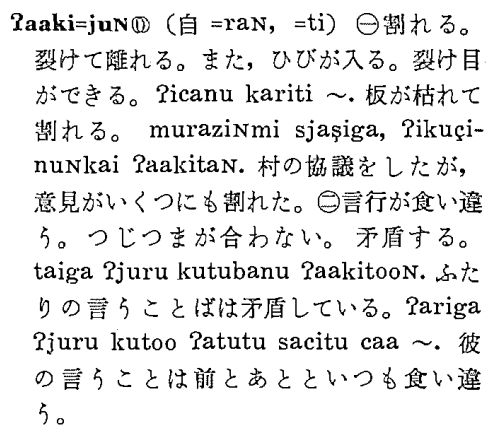
\includegraphics[height=0.5\paperheight,width=0.4\paperwidth]{oki-dict-example-aakiyun-original.png}
        %\caption{PDF}
      \end{minipage}%
      \begin{minipage}{0.5\textwidth}
        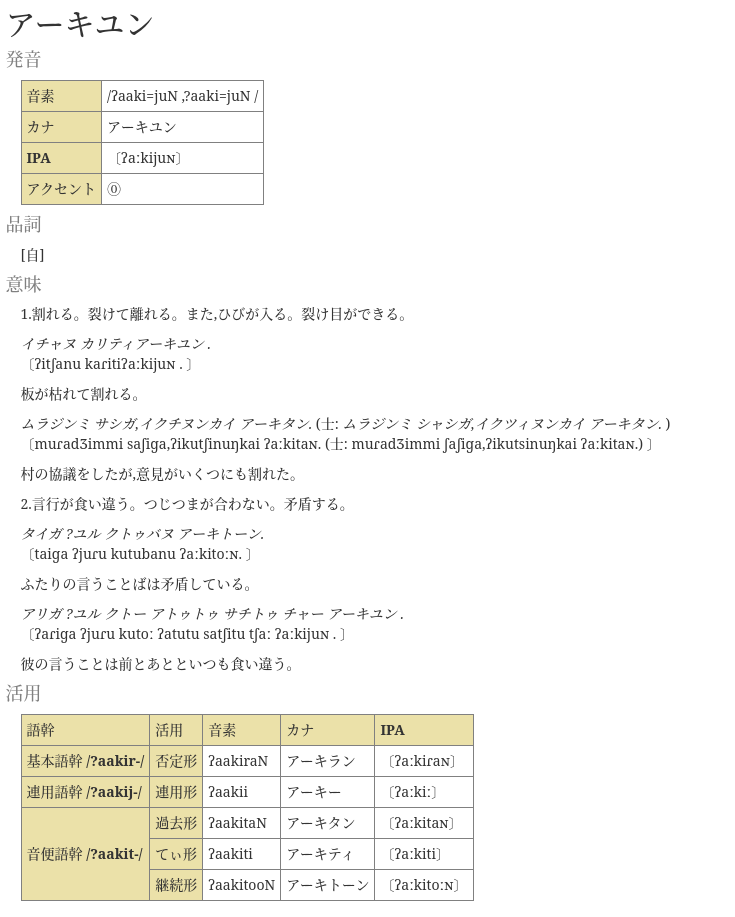
\includegraphics[height=0.65\paperheight]{oki-dict-example-aakiyun-online.png}
        %\caption{オンライン沖縄語辞典}
      \end{minipage}
    \end{figure}
  \end{block}
\end{frame}

\begin{frame}{オンライン沖縄語辞典の紹介}
  \begin{block}{見出し語・例文をカナ表記}
    \begin{itemize}
    \item 沖縄語音素表記を音節に分解し、カナに変換する処理を実装。
    \item カナ表記は可能な限り多様な表記法に対応
    \item 士族発音がある場合は併記。(「解説篇」を参照した)
    \item 副産物として、沖縄語音素表記の誤表記を検出できるようになった。
    \end{itemize}
  \end{block}
\end{frame}
% \end{frame}
\begin{frame}{オンライン沖縄語辞典の紹介}
  \begin{block}{解説文と例文の分離}
    \begin{itemize}
    \item 説明文内の日本語のパラグラフと沖縄語の例文(音素表記)とを分解する処理を実装。
    \item ユニットテストと音素カナ変換のエラー検知機能を使いトライ&エラーで適切な正規表現を作成。
    \item 「ほとんど」の例文を分離できているが、一部できていない箇所もあるかもしれない。正規表現による正確な処理は対象データに対する網羅的な知識が必要。
    \end{itemize}
  \end{block}
\end{frame}
\begin{frame}{オンライン沖縄語辞典の紹介}
  \begin{block}{動詞活用表の生成}
    \begin{itemize}
    \item 元の『沖縄語辞典』では品詞の部分に否定形とティ形語幹末尾のみの記載だった。
    \item 不規則動詞の活用辞書を手で作成。規則動詞は自動生成。
    \end{itemize}
    \begin{figure}[ht]
      \centering
      \begin{minipage}{0.4\paperwidth}
        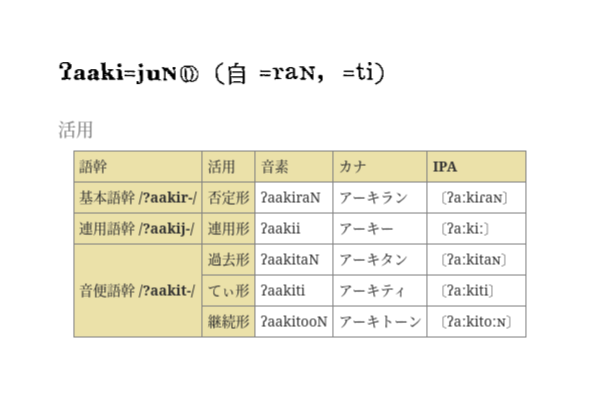
\includegraphics[height=0.36\paperheight]{verb-conugation-comparison.png}
        %\caption{PDF}
      \end{minipage}%
      \begin{minipage}{0.4\textwidth}
        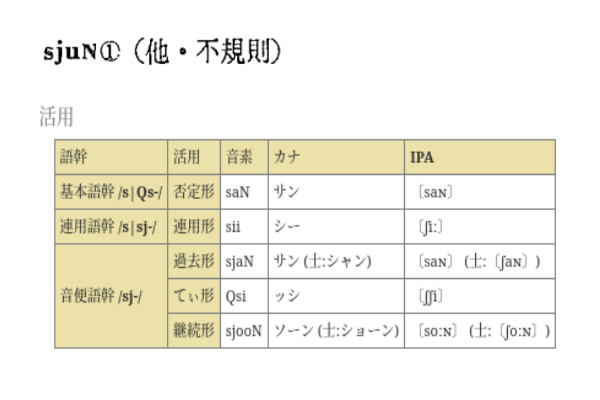
\includegraphics[height=0.34\paperheight]{verb-conjugation-comparison-2.png}
        %\caption{オンライン沖縄語辞典}
      \end{minipage}
    \end{figure}
  \end{block}
\end{frame}
%---------  うちなーぐち活用辞典 ----------% 
\begin{frame}{オンライン沖縄語辞典の紹介}
  \begin{block}{うちなーぐち活用辞典}
    \begin{itemize}
    \item 
    \item PDF の構造化されていないデータを文字のフォント・色・位置・大きさなどの情報からマニュアルで構造化
    \end{itemize}
    \begin{figure}[ht]
      \centering
      \begin{minipage}{0.4\paperwidth}
        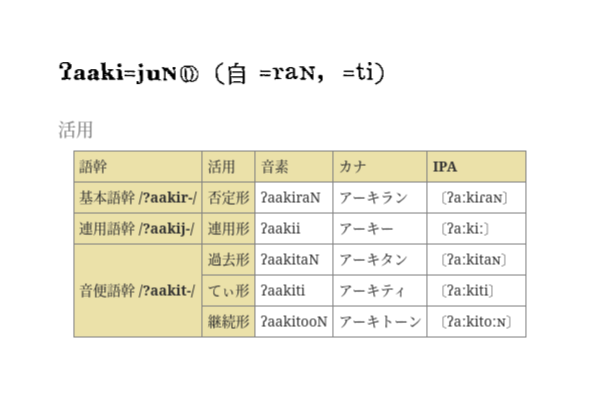
\includegraphics[height=0.36\paperheight]{verb-conugation-comparison.png}
        %\caption{PDF}
      \end{minipage}%
    \end{figure}
  \end{block}
\end{frame}
%---------  知見 ----------% 
\begin{frame}{開発から得た知見}
  \begin{block}{アクセシビリティ(accessibility)の重要性}%
    \vspace{0pt}
    アクセシビリティ := アクセスのしやすさとは...
    \begin{itemize}
    \item 見つけやすさ(searchability)
      \begin{itemize}
        \item すぐに見つけられる。
      \end{itemize}
    \item 入手しやすさ(reachability)
      \begin{itemize}
      \item 街の本屋、図書館にある。高くない。
      \end{itemize}
    \item 使いやすさ(usability)
      \begin{itemize}
      \item 使いこなすのに特別な訓練を必要としない。
      \end{itemize}
    \item \textbf{利用する側からの視点が重要。}
    \end{itemize}
  \end{block}
\end{frame}
\begin{frame}{開発から得た知見}
  \begin{block}{XXにとって利用しやすいデータとは}
    \begin{itemize}
    \item 一般ユーザーにとって
      \begin{itemize}
      \item インターネットで検索ヒットしやすい。紙の書籍なら一般書店で購入可能である。
      \item 利用料が安価・無料。
      \item 使いやすい
      \end{itemize}
    \item 開発者にとって
      \begin{itemize}
      \item データがダウンロード可能で、ある程度構造化(Excel, CSV, JSON, etc)されている。
      \item ソースコードがレポジトリで公開されている。
      \end{itemize}
    \end{itemize}
  \end{block}
\end{frame}
%--------- 展望 ----------% 
\begin{frame}{今後の展望}
  \begin{block}{アプリの改良・充実}
    \begin{itemize}
    \item 辞書機能の充実(活用表の充実、お気に入り語彙、履歴、モバイルアプリ化等)
    \item 学習サポート機能(動詞活用練習、語彙暗記テスト等)
    \item 他辞書の取り込み(さらなる沖縄語、琉球諸語の辞書の追加)
    \item Wiki 作成
    \item 共同開発者・資金調達
    \end{itemize}
  \end{block}
\end{frame}
%--------- 終わり ----------% 
\begin{frame}{終わい}
  \begin{center}
  \LARGE{\ruby{終}{う}わいまでぃ\ruby{聞}{ち}ち\ruby{呉}{くぃ}みそーち\\いっぺー\ruby{御拝}{にふぇー}でーびる。}
  \end{center}
\end{frame}
\end{document}